\documentclass[11pt, oneside]{article}   	% use "amsart" instead of "article" for AMSLaTeX format
\usepackage{geometry}                		% See geometry.pdf to learn the layout options. There are lots.
\geometry{letterpaper}                   		% ... or a4paper or a5paper or ... 
%\geometry{landscape}                		% Activate for rotated page geometry
%\usepackage[parfill]{parskip}    		% Activate to begin paragraphs with an empty line rather than an indent
\usepackage{graphicx}				% Use pdf, png, jpg, or eps§ with pdflatex; use eps in DVI mode
\usepackage{amsmath}								% TeX will automatically convert eps --> pdf in pdflatex		
\usepackage{amssymb}
\usepackage[final]{pdfpages}

\title{HW 1.2}
\author{David Abramov}	

\begin{document}
\maketitle

\section{Resonance Curves for 3 Different Damping Coefficients}

$Q_{1}=$
$Q_{2}=$
$Q_{3}=$

There was no way to observe a shift in $\omega_{2}$ from my data because the mass was changed in order to achieve three different resonance curves. However, if I had kept the mass consistent for each trial and instead changed the relative position of the magnet in the stack of weights, then I would have been able to see a shift in $\omega_{2}$.  

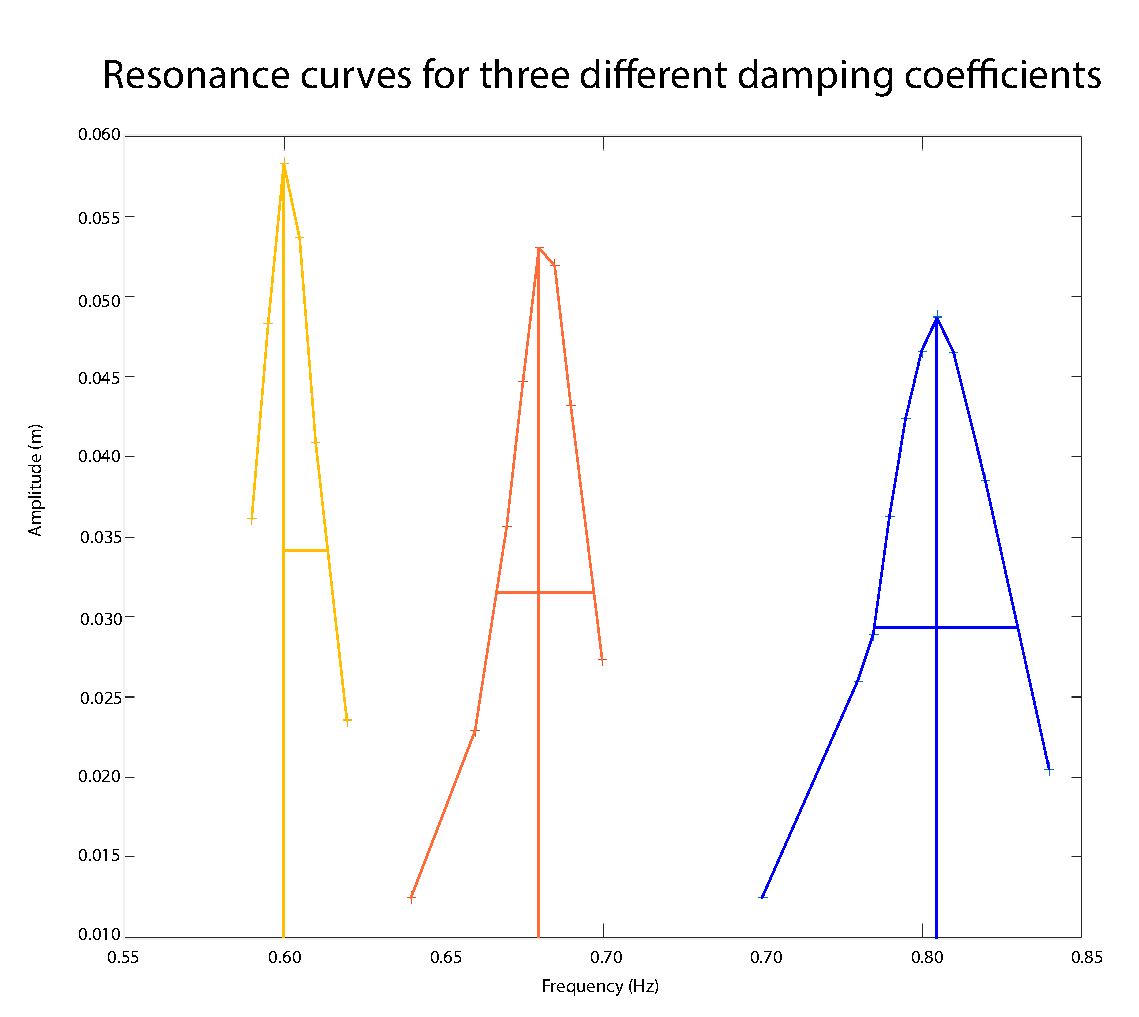
\includepdf[pages=-]{hwhm_h.pdf}

\section{Measuring Q in Other Ways}

I was able to measure Q in other ways by starting the measurement with the frequency set to $0.600$ Hz and then unplugging the wave generator, and also by starting the measurement with the wave generator unplugged and set to 0.600 Hz.

\section{Measuring small incremental changes in glider mass}

Data was collected for the same glider five times, each time with a different number of 5 g masses (ranging from 0 to 4).

\end{document}